%
% This is the LaTeX template file for lecture notes for CS294-8,
% Computational Biology for Computer Scientists.  When preparing 
% LaTeX notes for this class, please use this template.
%
% To familiarize yourself with this template, the body contains
% some examples of its use.  Look them over.  Then you can
% run LaTeX on this file.  After you have LaTeXed this file then
% you can look over the result either by printing it out with
% dvips or using xdvi.
%
% This template is based on the template for Prof. Sinclair's CS 270.

\documentclass[twoside]{article}
\usepackage{graphics}
\usepackage{amsfonts}
\usepackage{tikz}
\setlength{\oddsidemargin}{0.25 in}
\setlength{\evensidemargin}{-0.25 in}
\setlength{\topmargin}{-0.6 in}
\setlength{\textwidth}{6.5 in}
\setlength{\textheight}{8.5 in}
\setlength{\headsep}{0.75 in}
\setlength{\parindent}{0 in}
\setlength{\parskip}{0.1 in}

%
% The following commands set up the lecnum (lecture number)
% counter and make various numbering schemes work relative
% to the lecture number.
%
\newcounter{lecnum}
\renewcommand{\thepage}{\thelecnum-\arabic{page}}
\renewcommand{\thesection}{\thelecnum.\arabic{section}}
\renewcommand{\theequation}{\thelecnum.\arabic{equation}}
\renewcommand{\thefigure}{\thelecnum.\arabic{figure}}
\renewcommand{\thetable}{\thelecnum.\arabic{table}}

%
% The following macro is used to generate the header.
%
\newcommand{\chno}[4]{
   \pagestyle{headings}
   \thispagestyle{plain}
   \newpage
   \setcounter{lecnum}{#1}
   \setcounter{page}{1}
   \noindent
   \begin{center}
   \framebox{
      \vbox{\vspace{2mm}
    \hbox to 6.28in { {\bf CS 378 Intro to Theory of Computation
                        \hfill Fall 2015} }
       \vspace{4mm}
       \hbox to 6.28in { {\Large \hfill Chapter #1: #2  \hfill} }
       \vspace{2mm}
       \hbox to 6.28in { {\it Professor #3 \hfill #4} }
      \vspace{2mm}}
   }
   \end{center}
   \markboth{Lecture #1: #2}{Lecture #1: #2}
   {\bf NB}: {\it These notes are a revised version of those taken during Dale Skrein's CS 378 course at Colby College in Fall 2015.  The course followed Michael Sipser's \textit{Introduction to the Theory of Computation (3ed)} text.}
   \vspace*{4mm}
}

%
% Convention for citations is authors' initials followed by the year.
% For example, to cite a paper by Leighton and Maggs you would type
% \cite{LM89}, and to cite a paper by Strassen you would type \cite{S69}.
% (To avoid bibliography problems, for now we redefine the \cite command.)
% Also commands that create a suitable format for the reference list.
\renewcommand{\cite}[1]{[#1]}
\def\beginrefs{\begin{list}%
        {[\arabic{equation}]}{\usecounter{equation}
         \setlength{\leftmargin}{2.0truecm}\setlength{\labelsep}{0.4truecm}%
         \setlength{\labelwidth}{1.6truecm}}}
\def\endrefs{\end{list}}
\def\bibentry#1{\item[\hbox{[#1]}]}

%Use this command for a figure; it puts a figure in wherever you want it.
%usage: \fig{NUMBER}{SPACE-IN-INCHES}{CAPTION}
\newcommand{\fig}[3]{
			\vspace{#2}
			\begin{center}
			Figure \thelecnum.#1:~#3
			\end{center}
	}
% Use these for theorems, lemmas, proofs, etc.
\newtheorem{theorem}{Theorem}[lecnum]
\newtheorem{lemma}[theorem]{Lemma}
\newtheorem{proposition}[theorem]{Proposition}
\newtheorem{claim}[theorem]{Claim}
\newtheorem{corollary}[theorem]{Corollary}
\newtheorem{definition}[theorem]{Definition}
\newenvironment{proof}{{\bf Proof:}}{\hfill\rule{2mm}{2mm}}

% **** IF YOU WANT TO DEFINE ADDITIONAL MACROS FOR YOURSELF, PUT THEM HERE:

\begin{document}
%FILL IN THE RIGHT INFO.
%\lecture{**LECTURE-NUMBER**}{**DATE**}{**LECTURER**}{**SCRIBE**}
\chno{1}{Regular Languages}{Dale Skrien}{Zach Schutzman}
%\footnotetext{These notes are partially based on those of Nigel Mansell.}

% **** YOUR NOTES GO HERE:

% Some general latex examples and examples making use of the
% macros follow.  
%**** IN GENERAL, BE BRIEF. LONG SCRIBE NOTES, NO MATTER HOW WELL WRITTEN,
%**** ARE NEVER READ BY ANYBODY.


\section{Languages}

Theory of Computation is the study of models of computation and what kind of problems those models can and cannot solve.  We will build from the simplest models of computation to more complex ones, until we reach models that can solve the same problems as modern computers.

\definition {An \textbf{alphabet} is a finite set of \textit{characters}.}

In this course, we will commonly use as our alphabet $\{0,1\}$ and $\{a,b\}$ in consideration of modern computing being built on binary representations of data.  Sometimes, however, we might want to consider an alphabet with more symbols, such as $\{0,1,2\}$, or the entire English alphabet $\{a,b,c,d\dots z\}$ or an extended unicode alphabet.  We usually denote our alphabet $\Sigma$.  We denote the set of all strings on the alphabet $\Sigma^{*}$.  More about the $\ ^{*}$ operator will come when we learn about regular expressions.

\definition {A \textbf{string} is an ordered collection of characters from $\Sigma$.  A string is finite in length.}

\definition {A \textbf{language} is a subset of $\Sigma^{*}$.  Equivalently, a language is a set of strings on an alphabet $\Sigma$.}

Just for clarity's sake, let's be explicit: $\Sigma$ is a finite set.  $\Sigma^{*}$ is a countably infinite set of finite sets.  An individual language is some subset of $\Sigma^{*}$, so it is at most countable. The number of languages on an alphabet $\Sigma$ is equal to the size of the power set of $\Sigma^{*}$.  This set is uncountably infinite.

\section{Deterministic Finite Automata}

Consider the following directed graph.  

\begin{center}
	\begin{tikzpicture}[scale=0.2]
	\tikzstyle{every node}+=[inner sep=0pt]
	\draw [black] (17.5,-25.3) circle (3);
	\draw (17.5,-25.3) node {$start$};
	\draw [black] (32.4,-25.3) circle (3);
	\draw (32.4,-25.3) node {$q_1$};
	\draw [black] (46.7,-25.3) circle (3);
	\draw (46.7,-25.3) node {$q_2$};
	\draw [black] (61.8,-25.3) circle (3);
	\draw (61.8,-25.3) node {$final$};
	\draw [black] (61.8,-25.3) circle (2.4);
	\draw [black] (12.3,-25.3) -- (14.5,-25.3);
	\fill [black] (14.5,-25.3) -- (13.7,-24.8) -- (13.7,-25.8);
	\draw [black] (20.5,-25.3) -- (29.4,-25.3);
	\fill [black] (29.4,-25.3) -- (28.6,-24.8) -- (28.6,-25.8);
	\draw (24.95,-24.8) node [above] {$1$};
	\draw [black] (31.077,-22.62) arc (234:-54:2.25);
	\draw (32.4,-18.05) node [above] {$0$};
	\fill [black] (33.72,-22.62) -- (34.6,-22.27) -- (33.79,-21.68);
	\draw [black] (16.177,-22.62) arc (234:-54:2.25);
	\draw (17.5,-18.05) node [above] {$0$};
	\fill [black] (18.82,-22.62) -- (19.7,-22.27) -- (18.89,-21.68);
	\draw [black] (35.4,-25.3) -- (43.7,-25.3);
	\fill [black] (43.7,-25.3) -- (42.9,-24.8) -- (42.9,-25.8);
	\draw (39.55,-24.8) node [above] {$1$};
	\draw [black] (45.377,-22.62) arc (234:-54:2.25);
	\draw (46.7,-18.05) node [above] {$0$};
	\fill [black] (48.02,-22.62) -- (48.9,-22.27) -- (48.09,-21.68);
	\draw [black] (49.7,-25.3) -- (58.8,-25.3);
	\fill [black] (58.8,-25.3) -- (58,-24.8) -- (58,-25.8);
	\draw (54.25,-24.8) node [above] {$1$};
	\draw [black] (60.477,-22.62) arc (234:-54:2.25);
	\draw (61.8,-18.05) node [above] {$0,1$};
	\fill [black] (63.12,-22.62) -- (64,-22.27) -- (63.19,-21.68);
	\end{tikzpicture}
\end{center}



Given some string $w$ on ${0,1}$, we begin at the start state and read each character of $w$ one at a time, following the appropriate arrow to the next state (possibly the same one).  

\definition {An automaton \textbf{accepts} a string if and only if stepping through the automaton ends in a \textbf{final} or \textbf{accept state}.  The language accepted by an automaton is exactly the set of strings on $\Sigma$ whose traversals end in a final state.  We say that an automaton \textbf{rejects} any string it does not accept.  For an automaton $M$, we denote the language that $M$ accepts as $\mathcal{L}(M)$.}

The above automaton accepts all strings on $\Sigma$ that have at least three $1$s.

Let's formalize this kind of automaton.

\definition {A \textbf{deterministic finite automaton}, or DFA, is formally a five-tuple $(Q,\Sigma , \delta , q_0, F)$
	
	\begin{enumerate}
		\item[] $Q$ is the set of states, and is finite.
		\item[] $\Sigma$ is an alphabet.
		\item[] $\delta$ is the transition function, which maps the current state and character to the next state.  
		\item[] $q_0$ is the start state and is an element of $Q$.
		\item[] $F$ is the set of final states and is a subset of $Q$.
		
	\end{enumerate}
		
}

\definition {A language is \textbf{regular} if an only if there exists some DFA which accepts it.}

This is our first (of many) definition of a regular language.  Now, the question arises of whether \textit{every} language is regular (obviously not, or this class wouldn't have much to talk about).

\claim {There exist non-regular languages.}

\begin{proof}
	Recall that we showed that the number of languages on an alphabet $\Sigma$ is uncountably infinite.  Note that in the definition of a DFA, we have a finite set of states $Q$, and a finite alphabet $\Sigma$, so $\delta$ must be finite as well, and all can be indexed by the natural numbers.  Therefore, the number of possible DFAs is in bijection with $\mathbb{N}\times\mathbb{N}\times\mathbb{N}$ and is therefore countable.  Therefore, there exist (uncountably many) non-regular languages.
\end{proof}

By the end of the chapter, we will have identified and constructed some non-regular languages.

Drawing the state diagram for a DFA is not always practical or feasible.  Consider the language on ${0,1}$ where each character appears exactly $100$ times.  Because DFAs read their inputs exactly once, this DFA requires over $10,000$ states to define.  Below is a DFA accepting the language of strings where each character appears exactly twice.

\begin{center}
	\begin{tikzpicture}[scale=0.2]
	\tikzstyle{every node}+=[inner sep=0pt]
	\draw [black] (22.6,-44.3) circle (3);
	\draw (22.6,-44.3) node {$start$};
	\draw [black] (36.2,-44.3) circle (3);
	\draw [black] (49.3,-44.3) circle (3);
	\draw [black] (22.6,-33.3) circle (3);
	\draw [black] (22.6,-21.1) circle (3);
	\draw [black] (36.2,-33.3) circle (3);
	\draw [black] (49.3,-33.3) circle (3);
	\draw [black] (36.2,-21.1) circle (3);
	\draw [black] (49.3,-21.1) circle (3);
	\draw (49.3,-21.1) node {$final$};
	\draw [black] (49.3,-21.1) circle (2.4);
	\draw [black] (36.2,-9.4) circle (3);
	\draw (36.2,-9.4) node {$reject$};
	\draw [black] (62.9,-33.3) circle (3);
	\draw (62.9,-33.3) node {$reject$};
	\draw [black] (15.8,-44.3) -- (19.6,-44.3);
	\fill [black] (19.6,-44.3) -- (18.8,-43.8) -- (18.8,-44.8);
	\draw [black] (25.6,-44.3) -- (33.2,-44.3);
	\fill [black] (33.2,-44.3) -- (32.4,-43.8) -- (32.4,-44.8);
	\draw (29.4,-44.8) node [below] {$1$};
	\draw [black] (39.2,-44.3) -- (46.3,-44.3);
	\fill [black] (46.3,-44.3) -- (45.5,-43.8) -- (45.5,-44.8);
	\draw (42.75,-44.8) node [below] {$1$};
	\draw [black] (22.6,-41.3) -- (22.6,-36.3);
	\fill [black] (22.6,-36.3) -- (22.1,-37.1) -- (23.1,-37.1);
	\draw (23.1,-38.8) node [right] {$0$};
	\draw [black] (22.6,-30.3) -- (22.6,-24.1);
	\fill [black] (22.6,-24.1) -- (22.1,-24.9) -- (23.1,-24.9);
	\draw (22.1,-27.2) node [left] {$0$};
	\draw [black] (25.6,-33.3) -- (33.2,-33.3);
	\fill [black] (33.2,-33.3) -- (32.4,-32.8) -- (32.4,-33.8);
	\draw (29.4,-33.8) node [below] {$1$};
	\draw [black] (36.2,-41.3) -- (36.2,-36.3);
	\fill [black] (36.2,-36.3) -- (35.7,-37.1) -- (36.7,-37.1);
	\draw (36.7,-38.8) node [right] {$0$};
	\draw [black] (49.3,-41.3) -- (49.3,-36.3);
	\fill [black] (49.3,-36.3) -- (48.8,-37.1) -- (49.8,-37.1);
	\draw (49.8,-38.8) node [right] {$0$};
	\draw [black] (39.2,-33.3) -- (46.3,-33.3);
	\fill [black] (46.3,-33.3) -- (45.5,-32.8) -- (45.5,-33.8);
	\draw (42.75,-33.8) node [below] {$1$};
	\draw [black] (36.2,-30.3) -- (36.2,-24.1);
	\fill [black] (36.2,-24.1) -- (35.7,-24.9) -- (36.7,-24.9);
	\draw (36.7,-27.2) node [right] {$0$};
	\draw [black] (49.3,-30.3) -- (49.3,-24.1);
	\fill [black] (49.3,-24.1) -- (48.8,-24.9) -- (49.8,-24.9);
	\draw (49.8,-27.2) node [right] {$0$};
	\draw [black] (25.6,-21.1) -- (33.2,-21.1);
	\fill [black] (33.2,-21.1) -- (32.4,-20.6) -- (32.4,-21.6);
	\draw (29.4,-21.6) node [below] {$1$};
	\draw [black] (39.2,-21.1) -- (46.3,-21.1);
	\fill [black] (46.3,-21.1) -- (45.5,-20.6) -- (45.5,-21.6);
	\draw (42.75,-21.6) node [below] {$1$};
	\draw [black] (24.87,-19.14) -- (33.93,-11.36);
	\fill [black] (33.93,-11.36) -- (32.99,-11.5) -- (33.65,-12.26);
	\draw (30.41,-15.74) node [below] {$0$};
	\draw [black] (36.2,-18.1) -- (36.2,-12.4);
	\fill [black] (36.2,-12.4) -- (35.7,-13.2) -- (36.7,-13.2);
	\draw (36.7,-15.25) node [right] {$0$};
	\draw [black] (47.06,-19.1) -- (38.44,-11.4);
	\fill [black] (38.44,-11.4) -- (38.7,-12.3) -- (39.37,-11.56);
	\draw (43.76,-14.76) node [above] {$0$};
	\draw [black] (37.363,-6.647) arc (184.82444:-103.17556:2.25);
	\draw (41.85,-3.54) node [right] {$0,1$};
	\fill [black] (39.09,-8.65) -- (39.93,-9.08) -- (39.85,-8.08);
	\draw [black] (51.53,-23.1) -- (60.67,-31.3);
	\fill [black] (60.67,-31.3) -- (60.41,-30.39) -- (59.74,-31.13);
	\draw (55.09,-27.69) node [below] {$1$};
	\draw [black] (52.3,-33.3) -- (59.9,-33.3);
	\fill [black] (59.9,-33.3) -- (59.1,-32.8) -- (59.1,-33.8);
	\draw (56.1,-33.8) node [below] {$1$};
	\draw [black] (51.63,-42.41) -- (60.57,-35.19);
	\fill [black] (60.57,-35.19) -- (59.63,-35.3) -- (60.26,-36.08);
	\draw (57.11,-39.29) node [below] {$1$};
	\draw [black] (65.228,-31.427) arc (156.54625:-131.45375:2.25);
	\draw (70.24,-31.46) node [right] {$0,1$};
	\fill [black] (65.8,-34.01) -- (66.34,-34.79) -- (66.74,-33.87);
	\end{tikzpicture}
\end{center}


The two states labeled \textit{reject} are often called \textbf{sinks}.  Any string whose traversal enters a sink is not in $\mathcal{L}(M)$.

Even if we cannot explicitly draw such a DFA, it is not hard to precisely describe what it might look like and assert that it exists.  A formal proof that the language of strings that have exactly $x_i$ occurrences of character $i$ proceeds by induction on the $x_i$.  For two characters, the DFA looks rectangular, for 3 characters it looks like a cube, and beyond that it becomes hard to visualize.  Inductive constructions like these will prove very useful moving forward.


\claim {The \textbf{empty language}, denoted $\emptyset$, and $\Sigma^*$ are regular languages.}

\begin{proof}
	The empty language is the empty set of strings on an alphabet.  Any DFA with no accept states by definition does not accept any strings, and therefore accepts the empty language.  Similarly, a DFA where all states are accept states must accept every string on the alphabet, which is the definition of the set $\Sigma^*$.
\end{proof}


\definition {The \textbf{union} of two languages $A$ and $B$, denoted $A\cup B$, is the set of strings $x$ such that $x\in A$ or $x\in B$ (or both).  This works just like the definition of set union.}

\definition {The \textbf{intersection} of two languages $A$ and $B$, denoted $A\cap B$, is the set of strings $x$ such that $x\in A$ and $x\in B$.  (Same as set intersection).}

\definition {The \textbf{symmetric difference} of two languages $A$ and $B$ is the set of strings $x$ such that $x\in A$ or $x\in B$ but $x\notin A\cap B$.  Symbolically, the symmetric difference is $A\cup B \backslash A\cap B$. (Follows from definition of symmetric difference of two sets.)}

\definition {The \textbf{reverse} of a language $\mathcal{L}$, denoted $\mathcal{L}^R$ is the set of strings $x^r = x_k x_{k-1} \dots x_1$ such that $x = x_1 x_2 \dots x_{k-1} x_k$ is a string in $\mathcal{L}.$}

\definition {The \textbf{complement} of a language $\mathcal{L}$, denoted $\mathcal{L}^C$ or $\bar{\mathcal{L}}$ is the set of strings $x\in\Sigma^*$ such that $x\notin\mathcal{L}$.}

\definition {The \textbf{concatenation} of two languages $A$ and $B$, denoted $A\circ B$ is the set of strings of the form $xy$, where $x\in A$ and $y\in B$.}

\definition {The \textbf{Kleene star} of a language $L$, written as $L^*$ (the same as in $\Sigma^*$) is the set of all strings $w$ such that $w$ is element of $L\circ L \circ \dots \circ L$ for some finite number of concatenations of $L$ with itself (including zero, i.e. $\epsilon\in L^*$).}

We're ready to prove our first real theorem about a property of regular languages.  It's going to turn out that the class of regular languages is closed under all seven of the operations above.  In probably a different order, we will prove this for union, reverse, complement, and concatenation.  Note that once we show closure under union and complement, DeMorgan's Laws gives us closure under intersection and symmetric difference for free, and the Kleene Star of a language is an inductive extension of concatenation.


\claim {The class of regular languages is closed under complement.  That is, the complement of a regular language is regular.}

\begin{proof}
	
	
	Recall that a language is regular if and only if a DFA accepts it.  Given a DFA for a regular language $L$, we will construct a DFA that accepts exactly those strings on $\Sigma$ not in $L$, i.e. $L^C$.
	
	Given a DFA $M$ that accepts $L$, note that any string that is not in $L$ finishes its traversal of $M$ in a non-final state and any string that is in $L$ finishes its traversal in a final state.  Intuitively, constructing $\bar{M}$ to be a copy of $M$ where a state in $\bar{M}$ is a final state if and only if the corresponding state of $M$ is a non-final state, and a state in $\bar{M}$ is a non-final state if and only if the corresponding state in $M$ is a final state.
	
	To show that $\bar{M}$ accepts the complement of $L$, we must show that every string in $\Sigma^*$ is accepted by exactly one of $M$ or $\bar{M}$.  Let $w$ be a string in $\Sigma^*$  suppose (without loss of generality) that $w$ is accepted by $M$.  Then $w$ finishes its traversal in some final state $q_i$.  By construction, passing $w$ to $\bar{M}$ results in the traversal finishing in the corresponding non-final state $q_i$.  Therefore, $M$ and $\bar{M}$ together accept all of $\Sigma^*$ and no string is accepted by both, therefore $\bar{M}$ accepts $L^C$, which by definition must be regular.
\end{proof}


\section{Nondeterministic Finite Automata}

We know there are languages that are not regular.  Maybe we can find some by relaxing the definition of the DFA?  Suppose we relax the definition of the transition function $\delta$.  We allow multiple transitions leaving a state on the same character, not every state must have a transition on every character in  $\Sigma$, and transitions can happen without consuming an input character, called an $\epsilon$-transition.  These are called \textit{nondeterministic finite automata (NFAs)}, because we perform $\epsilon$-transitions and choices from among multiple transitions nondeterministically.


\begin{center}
	\begin{tikzpicture}[scale=0.2]
	\tikzstyle{every node}+=[inner sep=0pt]
	\draw [black] (22,-26.9) circle (3);
	\draw (22,-26.9) node {$start$};
	\draw [black] (34.2,-17.7) circle (3);
	\draw (34.2,-17.7) node {$q_1$};
	\draw [black] (34.2,-35.9) circle (3);
	\draw (34.2,-35.9) node {$q_2$};
	\draw [black] (47,-26.9) circle (3);
	\draw (47,-26.9) node {$q_3$};
	\draw [black] (60.2,-26.9) circle (3);
	\draw (60.2,-26.9) node {$final$};
	\draw [black] (60.2,-26.9) circle (2.4);
	\draw [black] (16.6,-26.9) -- (19,-26.9);
	\fill [black] (19,-26.9) -- (18.2,-26.4) -- (18.2,-27.4);
	\draw [black] (24.4,-25.09) -- (31.8,-19.51);
	\fill [black] (31.8,-19.51) -- (30.86,-19.59) -- (31.47,-20.39);
	\draw (29.1,-22.8) node [below] {$0$};
	\draw [black] (24.41,-28.68) -- (31.79,-34.12);
	\fill [black] (31.79,-34.12) -- (31.44,-33.24) -- (30.85,-34.05);
	\draw (26.35,-31.9) node [below] {$0,1$};
	\draw [black] (36.64,-19.45) -- (44.56,-25.15);
	\fill [black] (44.56,-25.15) -- (44.21,-24.28) -- (43.62,-25.09);
	\draw (39.6,-22.8) node [below] {$0$};
	\draw [black] (36.65,-34.17) -- (44.55,-28.63);
	\fill [black] (44.55,-28.63) -- (43.6,-28.68) -- (44.18,-29.49);
	\draw (41.52,-31.9) node [below] {$\epsilon$};
	\draw [black] (50,-26.9) -- (57.2,-26.9);
	\fill [black] (57.2,-26.9) -- (56.4,-26.4) -- (56.4,-27.4);
	\draw (53.6,-27.4) node [below] {$\epsilon,1$};
	\end{tikzpicture}
\end{center}


This is an NFA which includes multiple transitions and $\epsilon$-transitions.  Sometimes these aren't as intuitive to grasp as DFAs.  Let's note that if a string is unable to transition on the current input character, the string is rejected (we can think of an implied sink).  For example, there is no transition from $q_1$ on the character $1$, so a string currently in $q_1$ with the next character of $1$ is rejected.  Observe that whereas in a DFA the traversal of every string was unique, whereas in an NFA there could be more than one legal traversal.  For example, the string $00$ could go $start\rightarrow_0 q_1 \rightarrow_0 q_3 \rightarrow_\epsilon final$, where it is accepted, or $start \rightarrow_0 q_2 \rightarrow_\epsilon q_3 \rightarrow_\epsilon final$, where it is rejected because there is nowhere to transition on the remaining $0$.  So does this machine accept or reject $00$?  We say that an NFA accepts a string if and only if there exists \textit{at least one} valid traversal which consumes all input characters and ends in a final state.  Therefore, $00$ \textit{is} in the language of this machine.

Let's try to characterize the language accepted by this machine.  There is no transition out of the final state, so this machine doesn't accept any string longer than three characters, so it should be pretty simple to list out the strings it does accept:
\begin{enumerate}
	\item[] $00\epsilon$ = $00$
	\item[] $001$
	\item[] $0\epsilon\epsilon$ = $0$
	\item[] $0\epsilon 1$ = $01$
	\item[] $1\epsilon\epsilon$ = $1$
	\item[] $1\epsilon 1$ = $11$
\end{enumerate}

Note that the empty string is rejected and the strings $10$, $111$, $101$, $011$, $110$, $100$, $000$, and $010$ are not in the language, and together these lists form an exhaustive enumeration of the strings of length three or less, so we have fully characterized the language.  Note that this language is also regular (every finite language is regular), so we didn't just stumble upon an example of an NFA that is more powerful than DFAs.  Let's keep exploring.

\definition {Formally, a NFA is a 5-tuple $(Q,\Sigma ,\delta ,q_0, F)$.  $Q,\Sigma q_0,F$ are defined as in the formalization of a DFA.  The difference in these definitions is in the transition function $\delta$.}

The transition function $\delta$ for an NFA is a little tricker than that of a DFA.  Whereas in the DFA case, $\delta$ was a function which mapped a state and a character to another state, in the NFA case, $\delta$ maps a state and a character (now including the empty character $\epsilon$) to a \textit{set of states}.  In the example machine above, $\delta$ maps the pair $(start,0)$ to the set $\{q_1,q_2\}$.

Let's observe that DFAs (almost) satisfy the definition of NFAs, we just need to tweak the elements of the codomain of $\delta$ to be singleton sets of states instead of states themselves.  Thus, every DFA is also an NFA and the class of languages accepted by NFAs is a superset of the regular languages, but is it a proper superset?

The answer is no.  The class of languages accepted by NFAs is exactly the regular languages.  We will show this by demonstrating that any NFA can be transformed into a DFA accepting exactly the same language.

\claim {Any NFA can be transformed into a proper DFA that accepts the same language.}

\begin{proof}	Let $M$ be an NFA.  Suppose, without loss of generality, that $M$ contains both multiple transitions and $\epsilon$-transitions.  The key to this construction is that the transition function for a DFA maps characters and states to individual states whereas that of an NFA maps to sets of states.

Let $Q$ be the set of states in $M$ and $\delta$ the transition function.  We will define a new set of states $Q'$ for the DFA.  States of the DFA (elements of $Q'$) will correspond to subsets of $Q$ and a new transition function $\delta'$ for the DFA which will properly states in $Q'$ and characters in $\Sigma$ to states in $Q'$.  

First, we can construct $\delta$ as a table (remember, all the factor sets are finite, so $\delta$ still is as well).  Make a row for each state of $M$ and a column for each character in $\Sigma$, excluding $\epsilon$.  In each entry, list the states of $M$ that the row state can transition to on the column character in $M$, including any possible $\epsilon$-transitions.  For example, in the NFA pictured before, the entry at row $q_1$, column $0$ would be the set $\{q_3,final\}$.  If no transition is possible, the entry is $\emptyset$.
	
Now, we can fully construct the DFA. Let $q'_0$, the start state, correspond to the singleton set containing the start state of $M$.  Now, make a state in $Q'$ for each subset corresponding to a row, column entry in the transition table (we can make one for every subset of $Q$, but those which do not appear in the table are unreachable and therefore we don't need to include them in the DFA).

For each corresponding transition in $\delta$, construct a transition in $\delta'$ where a state $q'_i$ transitions to state $q'_j$ on character $k$ if and only if there exists a transition in $\delta$ from some state $a\in Q$ to $b\in Q$ on character $k$ where $a$ is an element of the subset corresponding to the state $q'_i$ and $b$ is in the subset corresponding to $q'_j$.  Finally, mark any state $q'_t$ a final state if and only if its corresponding subset of $Q$ contains at least one final state of $M$.  For sake of completeness and explicitness, the state corresponding to $\emptyset$ is a sink.

It is obvious that this new machine we constructed, call it $M'$, is a DFA, but it is not quite clear that $\mathcal{L}(M) = \mathcal{L}(M')$.  We will hand-wave a bit to claim that this equality in fact holds.

If $w$ is a string accepted by $M$, then there exists some valid traversal for $w$ ending in a final state.  Given such a traversal (an ordered list of states of $M$), we can construct the corresponding traversal in the DFA $M'$ by grouping the $\epsilon$-transitions in the travesral of $M$ into subsets with the preceding character transition (each subset is the character transition grouped with all immediately following $\epsilon$-transitions, if they exist), and mapping these subsets to the corresponding states in $M'$.  Since the traversal in $M$ ends in a final state, the traversal in $M'$ ends in a state corresponding to a subset containing a final state, and $M'$ accepts $w$.  Similarly, any string not accepted by $M$ ends its traversal in a non-final state of $M'$, or in the sink corresponding to $\emptyset$.  

Now let $x$ be a string accepted by $M'$.  Its accepting traversal in $Q'$ is unique, but the traversal in $M$ may not be.  The list of valid traversals in $M$ can be constructed by enumerating all of the paths generated by choosing one state from each of the subsets corresponding to the traversed states in $Q'$, where $\epsilon$-transitions are included with their preceding character transitions.  Since the traversal in $M'$ ends in a final state, at least one of the traversals in $M$ must end in a final state as well, and therefore $M$ accepts $x$.  A similar argument shows that strings not accepted in $M'$ are not accepted in $M$ either.

Therefore, $\mathcal{L}(M) =\mathcal{L}(M')$.

\end{proof}

\section{Proving Closure Properties}
	While NFAs are a little trickier to grasp than DFAs, they allow for non-deterministic (i.e. multiple and $\epsilon$) transitions, and since DFAs and NFAs accept the same class of language, we can prove things about regular languages by proving things about NFAs.
	
	\claim{The class of regular languages is closed under concatenation.}
	
	This is tricky to prove without non-determinism.  If we have two regular languages $A$, $B$ and some string, determining whether the string is in the concatenation $A\circ B$ is tricky.  We want to determine whether there is a way to split the string into two pieces so that the first part is in $A$ and the second part is in $B$, but we have no guidance on how to choose where to split the string.  It is possible that there are several possible ways to successfully split it, ways to split it such that the first part is in $A$ and the second part is not in $B$, or the other way around.  The string is in $A\circ B$ if there exists at least one valid split, but how do we choose which one?
	
	\begin{proof}
		
		Let $A$ and $B$ be regular languages and denote their concatenation by $A\circ B$.  We will construct an NFA that accepts $A\circ B$.
		
		Let $M_A$ be an NFA accepting $A$ and $M_B$ be an NFA accepting $B$.  Perform the following constructive modification:
		\begin{enumerate}
			\item For each final state in $M_A$, add an $\epsilon$-transition to the start state of $M_B$.
			\item Set the new final states to be only the final states of $M_B$.
			\item Set the new start state to be only the start state of $M_A$.
		\end{enumerate}
		
		This new machine accepts exactly the strings in $A\circ B$.  To see this, note that for the first part of the string to be in $A$, there must be at least one successful traversal that passes through one of the states that was originally a final h of $M_A$.  For the second part to be in $B$, the successful traversal must then make an $\epsilon$-transition to what was originally the start state of $M_B$ and then end in a final state.
		
		Since we now have an NFA to recognize $A \circ B$, it is regular, therefore the class of regular languages is closed under concatenation.
		
		
	\end{proof}
	
	
	\claim{The class of regular languages is closed under the Kleene Star operation.}
	
	The proof of this is similar to the previous one.  We will take an NFA that accepts a regular language $L$ and convert it to one that accepts $L^*$, which is the set of strings that are in some finite number of concatenations of $L$ with itself, including zero.
	
	
	\begin{proof}
		
		
		
		Let $L$ be a regular language and $M_L$ be an NFA (or DFA) that accepts it.  Perform the following constructive modification:
		
		\begin{enumerate}
			\item Make $\epsilon$-transitions from the final state of $M_L$ to the start state
			\item Make a new start state which is also a final state and add an $\epsilon$-transition to the original start state.			
			
		\end{enumerate}
		
		Note that this new machine accepts the empty string (zero concatenations of $L$ with itself), as well as non-deterministically allowing an arbitrary (finite) number of splits in the string.  If there is a valid way to split the string such that each part is in $L$, then it is in $L^*$ and this machine accepts it.
		
	\end{proof}



\claim{The class of regular languages is closed under union.}

We again perform a constructive modification to two NFAs accepting regular languages $A$ and $B$ to build one accepting $A\cup B$.  We want to somehow construct an NFA that simultaneously runs a string through $M_A$ and $M_B$ and accepts if and only if at least one of these machines accept.

\begin{proof}
	
	Let $A$ and $B$ be regular languages with NFAs $M_A$, $M_B$.  Add a new start state with $\epsilon$-transitions to the start states of $M_A$ and $M_B$, representing a non-deterministic choice of which language to check.  Since this new machine will accept if and only if at least one of $M_A$ and $M_B$ accept, it recognizes the union of the languages.
	
	
	
\end{proof}


\end{document}





